\documentclass[a4paper, oneside, nobib, notoc, justified]{tufte-book}

% Load packages
\usepackage{graphicx,xcolor}
\usepackage{tikz}
\pgfrealjobname{fig}
\usepackage{amsmath,amssymb}

% Colors
\definecolor{lightgray}{HTML}{D6D7D9}

% Commands
\newcommand{\ft}[0]{\footnotesize}
\newcommand{\scs}[0]{\scriptsize}
\newcommand{\sm}[0]{\small}
\newcommand{\degree}{\ensuremath{^\circ}}

\begin{document}
    \beginpgfgraphicnamed{fig1_04}
    \small
    \begin{tikzpicture}
        \draw (-3,0)      node {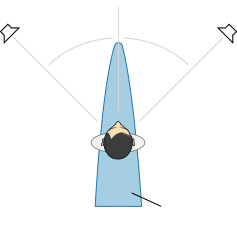
\includegraphics[width=.4\columnwidth]{src/stereo}};
        \draw (3,0)       node {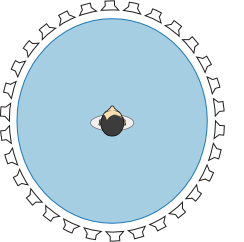
\includegraphics[width=.45\columnwidth]{src/sfs}};
        \draw (-3,3)      node {stereophony};
        \draw (3,3)       node {sound field synthesis};
        \draw (-3.6,0.7)  node {\color{lightgray}\ft $30\degree$};
        \draw (-2.35,0.7) node {\color{lightgray}\ft $30\degree$};
        \draw (-2,-1.93)  node {\ft sweet-spot};
    \end{tikzpicture}
    \endpgfgraphicnamed
\end{document}
